\section{Test Description and Success Criteria}
The unit test, test\_orb\_elem\_convert.py,  validates the internal aspects of the Basilisk orb\_elem\_convert module by comparing module output to expected output. The unit test validates the conversions performed between Keplerian orbital elements and Cartesian vectors. This test begins by converting elements to Cartesian and is immediately followed by converting the results back to orbital elements, providing the opportunity to compare the initial input with the final output. This is repeated for a variety of parameters. 

Differences between simulated and calculated output are measured, and those that approximately equal zero (typically $\delta < 10^{-9}$) qualify as a successful test. However, since the semimajor axis and the Cartesian vectors are greater than the other parameters by a factor of at least $10^7$, a higher discrepency is more tolerable. These tolerances are more clearly defined with the results.

\subsection{Element to Cartesian}
This test verifies the conversion from orbital elements to Cartesian vectors by comparing position and velocity vectors calculated in Python to those determined in the module. It uses six orbital elements and a gravitational constant as inputs. Also, \textit{Elements2Cart} and \textit{inputsGood} must be set to \textit{True}, which is discussed in more detail in the next section. The \textit{useEphemFormat} parameter is alternated between \textit{True} and \textit{False} to test the use of both spacecraft and planet data. The calculations for this conversion are performed seperately in the test module to compare with the simulated results. Multiple tests were performed, varying semimajor axis and eccentricity inputs.
\subsubsection{Calculation vs. Module}
The first check compares calculated Cartesian vectors to the simulated results and verifies that the discrepancy is less than $10^{-9}$.

\subsection{Cartesian to Element} 
This test verifies, via two checks, that the conversion from Cartesian vectors to orbital elements is accurate. This test requires position and velocity vectors, which are obtained through initially converting from orbital elements to Cartesian, as described above. It also needs a gravitational constant input. The \textit{Elements2Cart} is set to \textit{False} and \textit{inputsGood} must be set to \textit{True}. Like in the previous conversion test, \textit{useEphemFormat} is alternated between \textit{True} and \textit{False} to ensure that the Cartesian vectors can use both planet and spacecraft state data identically and accurately. The calculations for this conversion are also performed seperately in the test to compare with the simulated results.
\subsubsection{Calculation vs. Module}
Similar to the first conversion test, this check compares the calculated orbital elements to the elements obtained from the module.
\subsubsection{Input vs. Module}
This second check is performed last and compares the final result, comprised of orbital elements, with the orbital elements initially used as inputs for the first conversion test. This verifies that the two conversion processes can be combined to reattiain the original orbital elements.

\section{Test Parameters}

The previous description only briefly mentions the input parameters required to perform the tests on this module, so this section details the parameters further. In addition to the parameters being converted, the unit test requires inputs that identify which conversion is performed, what type of state data are being used, and whether or not to proceed with the given input. 

\begin{enumerate}
	\item \underline{Euler Angles}:\\
	Euler angles, consisting of $i$, $\Omega$, and $\omega$, define the orbit plane orientation and may vary, depending on the orbit type. All non-zero values for these angles were pulled from an existing module and are actually used in many other Basilisk tests in the SimScenarios directory. This parameter set gives the following inclination, ascending node, and argument of periapses inputs:
	\begin{equation}\label{eq:42}
		i = 33.3^{\circ} = 0.5812 \text{rad}
	\end{equation}
	\begin{equation}\label{eq:43}
		\Omega = 48.2^{\circ} = 0.8412 \text{rad}
	\end{equation}
	\begin{equation}\label{eq:44}
		\omega = 347.8^{\circ} = 6.0703 \text{rad}
	\end{equation}
	Inputs alternate between zero and these given values depending on the orbit type, which is specified in the results section. All angles must be input as radians, so the conversion from degrees is performed as shown in Eq. \ref{eq:42} - \ref{eq:44}.
	\item \underline{True Anomaly}:\\
	The true anomaly input stays the same for each parameter set because the different orbits do not require a unique value, as they may for inclination, ascending node, and argument of periapsis. The true anomaly value, however, is pulled from the same module as those parameters, giving 
	\begin{equation} \label{eq:41}
		f = 85.3^\circ = 1.489 \text{rad}
	\end{equation}
	\item \underline{Standard Gravitational Parameter}:\\
	The gravitational parameter $\mu$ is necessary for any conversion between orbital elements and Cartesian vectors. It is the product of a body's gravitational constant and mass, specifying the attracting body in units of $\frac{m^3}{s^2}$. This test specifies Earth as the astronomical body.
	\begin{equation}
		\mu = GM_{Earth}=3.986 \text{e+} 14\quad \frac{m^3}{s^2}
	\end{equation}
	\item \underline{Conversion Identifier}:\\
	In order to specify which conversion to perfom, that is Element to Cartesian or the reverse, an identifier must be set. In the test as well as the c++ file, this is a boolean flag, referred to as \textit{Elements2Cart} and indicating the cases displayed in the table below.
	\begin{table}[htbp]
		\caption{Elements2Cart Cases}
		\centering \fontsize{10}{10}\selectfont
		\begin{tabular}{c|c}
			\hline \textbf{Case} & \textbf{Conversion}\\ \hline True & Element to Cartesian\\ False & Cartesian to Element\\
			\hline
		\end{tabular}
	\end{table}
	\item \underline{Astronomical Body Identifier}\\
	Like the previous identifier, this is a boolean parameter that specifies how to use the module. Since the state data may describe any body in orbit, a value is needed to determine whether the conversions are being performed for a spacecraft or a planet. As stated previously, the test uses \textit{useEphemFormat} for this, providing the following options:
	\begin{table}[htbp]
		\caption{useEphemFormat Cases}
		\centering \fontsize{10}{10}\selectfont
		\begin{tabular}{c|c}
			\hline \textbf{Case} & \textbf{Body}\\ \hline True & Planet State Data\\ False & Spacecraft State Data\\
			\hline
		\end{tabular}
	\end{table}
	\item \underline{Valid Input Identifier}\\
	The last necessary parameter is another boolean flag, this time indicating whether the inputs are valid. This value is read from a message and distinguishes if it is written succesfully. If succesful, this allows the rest of the module to be run, initiating the conversion process. The test uses \textit{inputsGood} to execute this check where \textit{True} lets the module proceed and \textit{False} does not, so this value should always be \textit{True} for the module to execute properly.
\end{enumerate}	
The orbital element parameters are varied throughout the test to validate a range of orbits. Since the test performs both conversions consecutively and the Cartesian results depend on the Keplerian inputs, the position and velocity vectors used for the second conversion also vary. These parameters are discussed with the results in the next section.
\begin{table}[H]
	\caption{Error Tolerance-Note: Absolute Tolerance is abs(truth-value)}
	\centering \fontsize{10}{10}\selectfont
	\begin{tabular}{c|c|c}
		\hline \textbf{Test} & \textbf{Calc/Sim Tolerance} & \textbf{Input/Output Tolerance}\\ \hline $a$ & $10^{-9}$ km & $10^{-7}$ km\\ $e$ & $10^{-9}$ & $10^{-9}$\\
		$i$ & $10^{-9}$ rad & $10^{-9}$ rad\\
		$\Omega$ & $10^{-9}$ rad & $10^{-10}$ rad\\
		$\omega$ & $10^{-9}$ rad & $10^{-9}$ rad\\
		$f$ & $10^{-9}$ rad & $10^{-9}$ rad\\
		$\bm{r}$ & $10^{-9}$ km & N/A\\
		$\bm{v}$ & $10^{-9}$ $\frac{\text{km}}{\text{s}}$ & N/A\\
		\hline
	\end{tabular}
\end{table}

\section{Test Results}

All checks within test\_orb\_elem\_convert.py passed as expected with a tolerance limit of about $10^{-9}$. This means all comparisons should have a discrepancy of no more than $10^{-9}$. This may vary depending on the parameters in question, for example, when comparing the semimajor axis, since it is a factor of at least $10^4$ larger than the other parameters. The tables in this section show the results of each test for various parameters followed by descriptions of the parameter sets.

\begin{itemize}
	\item \textbf{Element to Cartesian}
	\begin{table}[H]
		\caption{Element to Cartesian Test Results}
		\label{tab:Cart to Elem results}
		\centering \fontsize{10}{10}\selectfont
		\begin{tabular}{c|c|c}
			\hline
			\textbf{Parameter Sets} & \textbf{Results} & \textbf{Notes} 									\\ \hline
			1 & \color{Green}{PASSED} & NA\\
			2 & \color{Green}{PASSED} & NA\\
			3 & \color{Green}{PASSED} & NA\\
			4 & \color{Green}{PASSED} & NA\\
			5 & \color{Green}{PASSED} & NA\\
			6 & \color{Green}{PASSED} & NA\\
			7 & \color{Green}{PASSED} & NA\\
			8 & \color{Green}{PASSED} & NA\\
			\hline
		\end{tabular}
	\end{table}
	Cartesian vectors are tested by comparing the simulated results of the conversion with calculated vectors. The discrepancy is expected to be no greater than $10^{-9}$ for both position and velocity. The two cases presented by the astronomical body identifier (\textit{useEphemFormat}), discussed in the Test Parameters section, produce identical results. Thus, they will not be referred to as seperate cases any further and only the various orbits will be analyzed. Plots comparing the position and velocity vectors are shown for each orbit. Only the upper and lower limits of the tests are displayed, providing insight into the effect of the changing parameters without an overwhelming amount of data.
	\begin{enumerate}
		\item \underline{Inclined Elliptic Orbit ($0<e<1.0$,\quad $a>0$)}\\
		To test elliptic orbtits, a range of semimajor axis inputs from $10-10^7$km is used. The eccentricity is also varied with inputs from $0.01-0.75$. As $a$ changes, $e=0.5$ and as $e$ changes, $a=10^7$km. All parameter sets passed for this case since the difference when comparing simulated and calculated results was always zero, as shown by Fig. \ref{fig:2} and \ref{fig:3}.
		\begin{figure}[H] 
			\centering
			\subfloat[$e=0.01$ and $a=10^7$km]{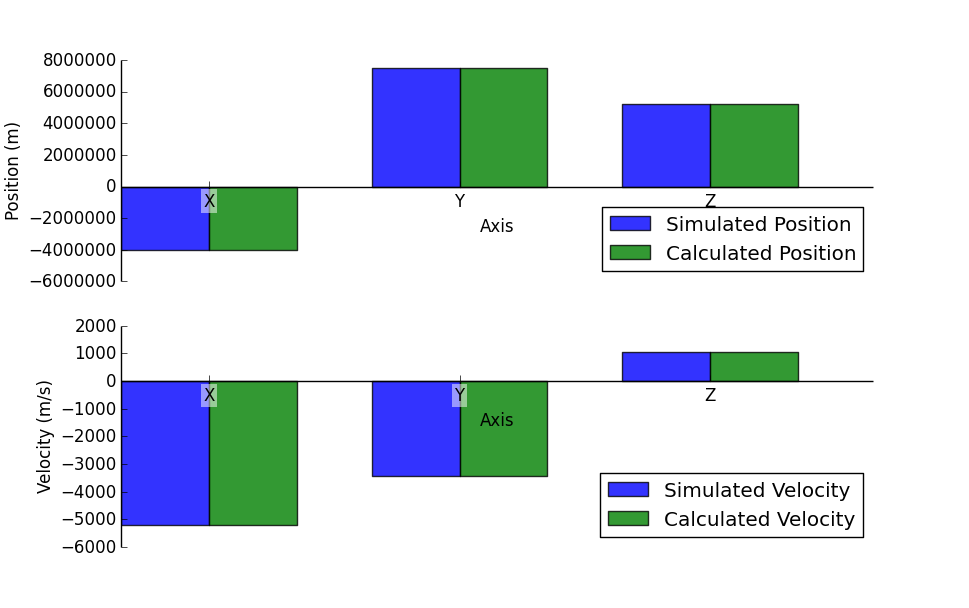
\includegraphics[width=0.5\textwidth]{Figures/IncEllipCart_e_1.png}}
			\subfloat[$e=0.75$ and $a=10^7$km]{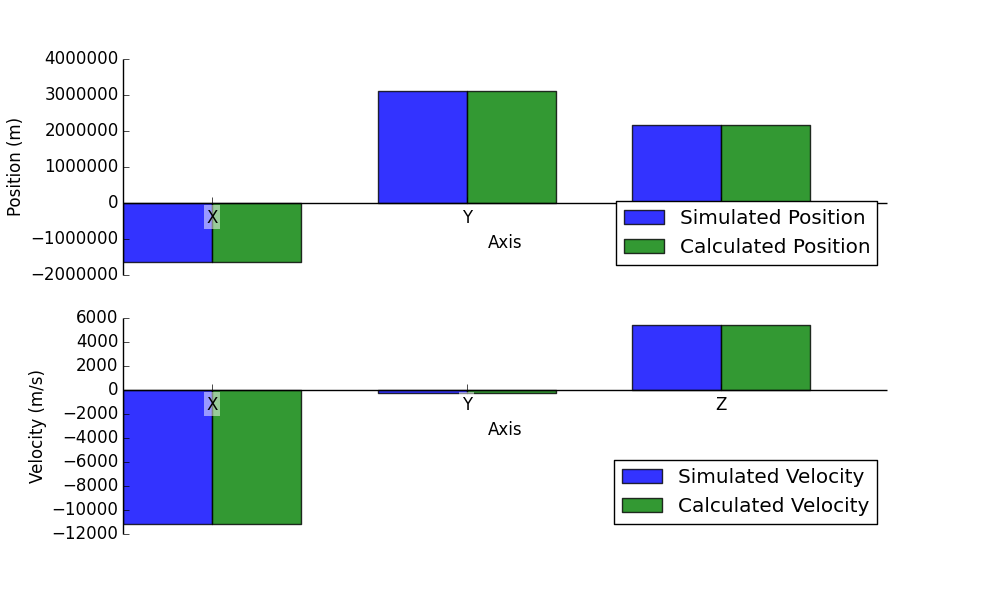
\includegraphics[width=0.5\textwidth]{Figures/IncEllipCart_e_2.png}}
			\caption{Inclined Elliptical Orbit Varying $e$}\label{fig:2}
		\end{figure}
		\begin{figure}[H]
			\centering
			\subfloat[$e=0.5$ and $a=10^7$km]{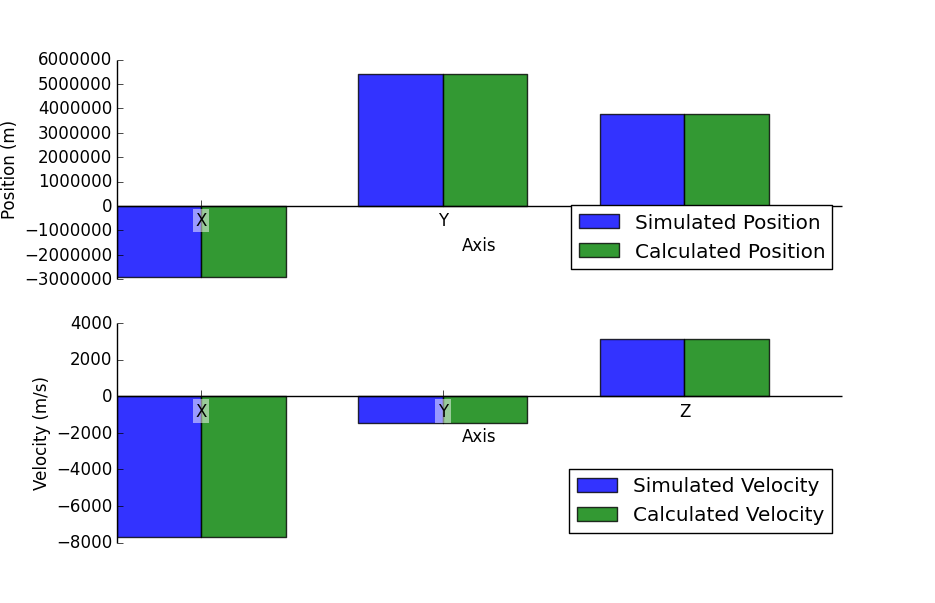
\includegraphics[width=0.5\textwidth]{Figures/IncEllipCart_a_1.png}}
			\subfloat[$e=0.5$ and $a=10$km]{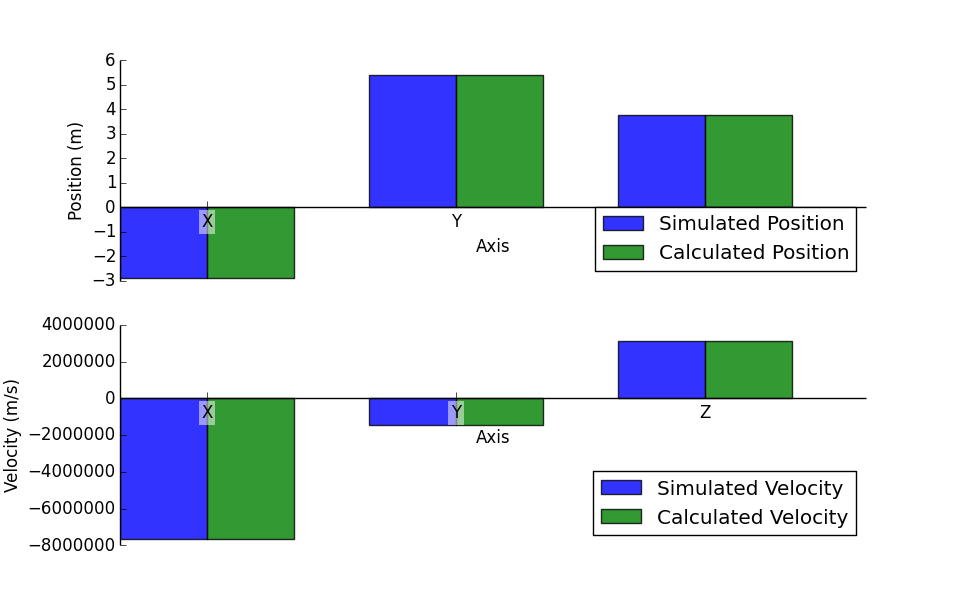
\includegraphics[width=0.5\textwidth]{Figures/IncEllipCart_a_2.png}}
			\caption{Inclined Elliptical Orbit Varying $a$}\label{fig:3}
		\end{figure}
		\pagebreak
		\item \underline{Equatorial Elliptic Orbit ($0<e<1.0$,\quad $a>0$,\quad $i=0$,\quad $\Omega=0$)}\\
		The equatorial elliptic orbit is tested with the same range of $e$ and $a$ inputs as the inclined case. All variations also passed this test with a tolerance of zero, as shown in the following set of figures:
		\begin{figure}[H] \label{fig:4}
			\centering
			\subfloat[$e=0.01$ and $a=10^7$km]{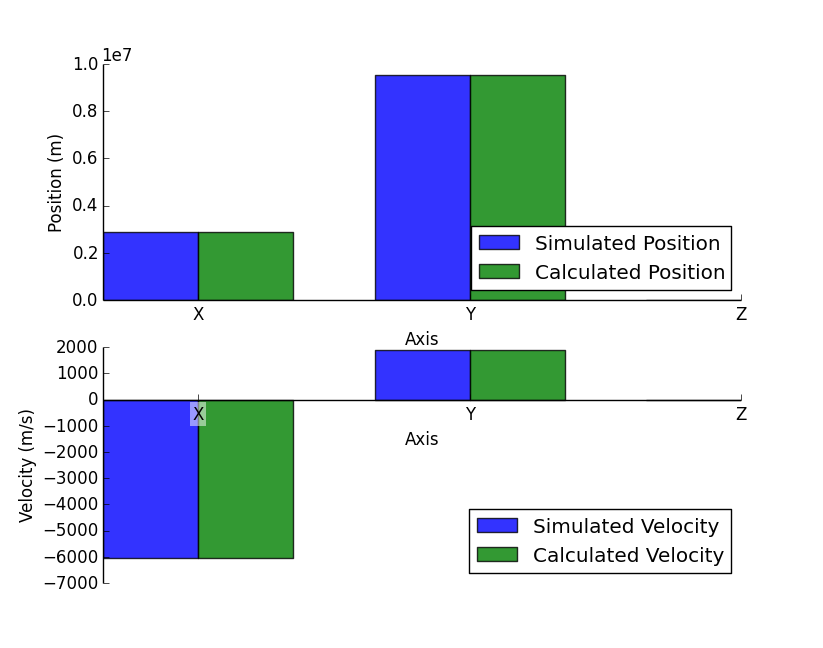
\includegraphics[width=0.5\textwidth]{Figures/EquEllipCart_e_1.png}}
			\subfloat[$e=0.75$ and $a=10^7$km]{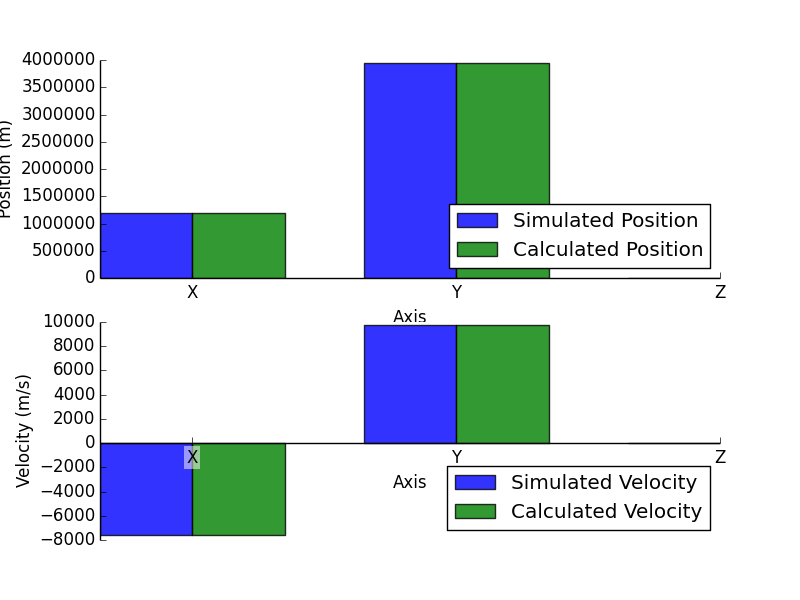
\includegraphics[width=0.5\textwidth]{Figures/EquEllipCart_e_2.png}}
			\caption{Equatorial Elliptical Orbit Varying $e$}
		\end{figure}
		\begin{figure}[H] \label{fig:5}
			\centering
			\subfloat[$e=0.5$ and $a=10^7$km]{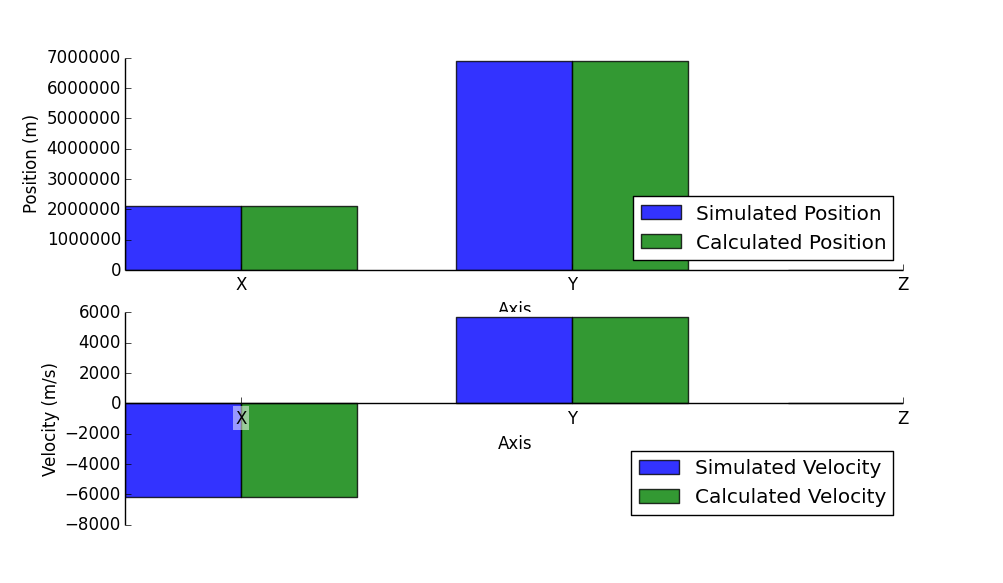
\includegraphics[width=0.5\textwidth]{Figures/EquEllipCart_a_1.png}}
			\subfloat[$e=0.5$ and $a=10$km]{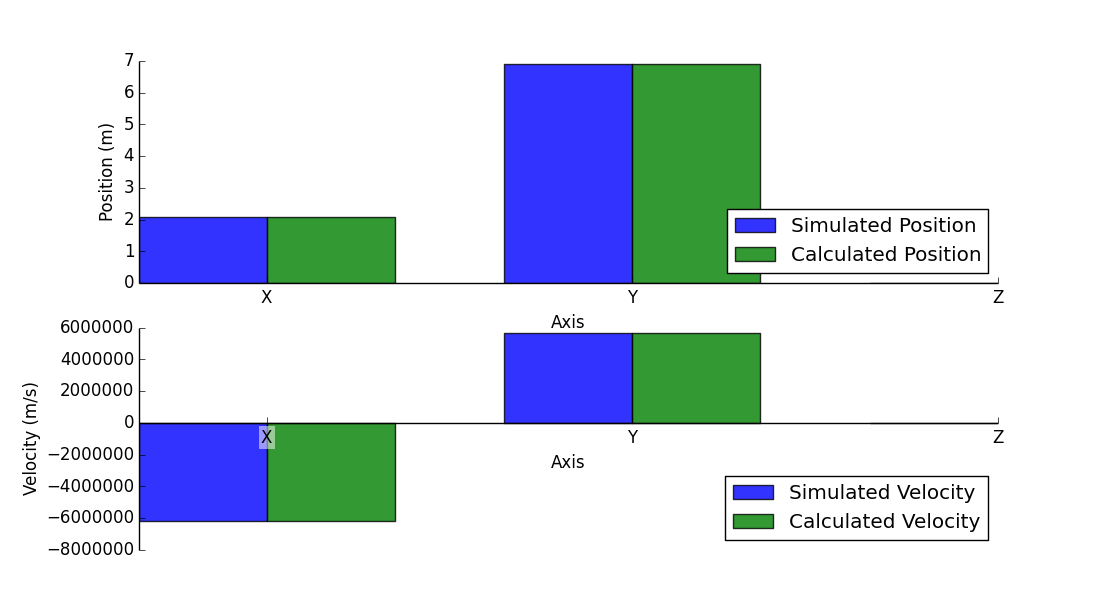
\includegraphics[width=0.5\textwidth]{Figures/EquEllipCart_a_2.png}}
			\caption{Equatorial Elliptical Orbit Varying $a$}
		\end{figure}
		\pagebreak
		\item \underline{Inclined Circular Orbit ($e=0$, \quad $a>0$,\quad $\omega=0$)}\\
		Since $e=0$ for a circular orbit, the only varied input is $a$, which is limited to the same range as in the elliptical cases. All variations passed for the inclined circular orbit, again, with no discrepancy.
		\begin{figure}[H] \label{fig:6}
			\centering
			\subfloat[$a=10^7$km]{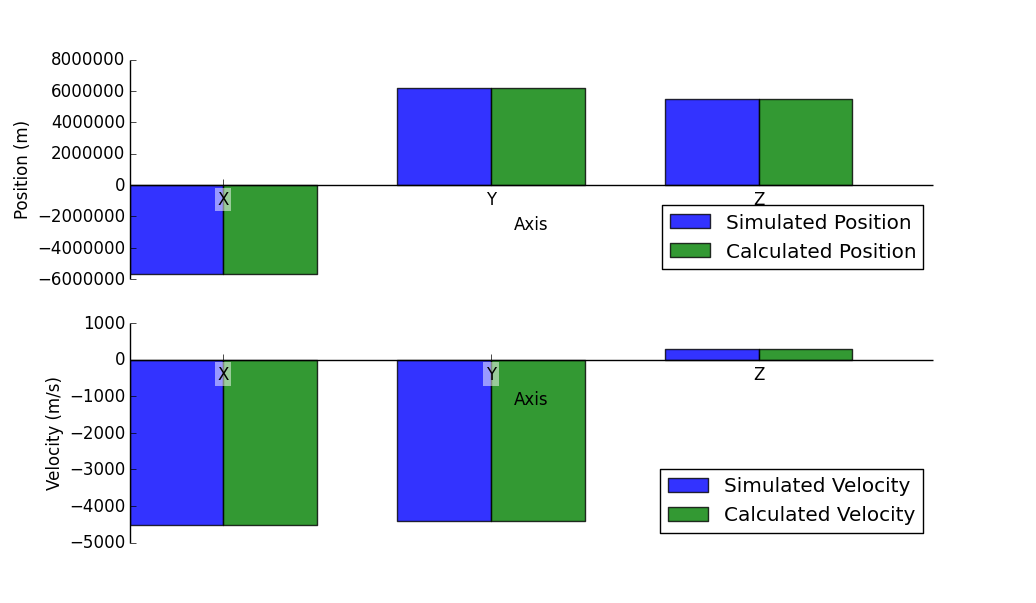
\includegraphics[width=0.5\textwidth]{Figures/IncCircCart_1.png}}
			\subfloat[$a=10$km]{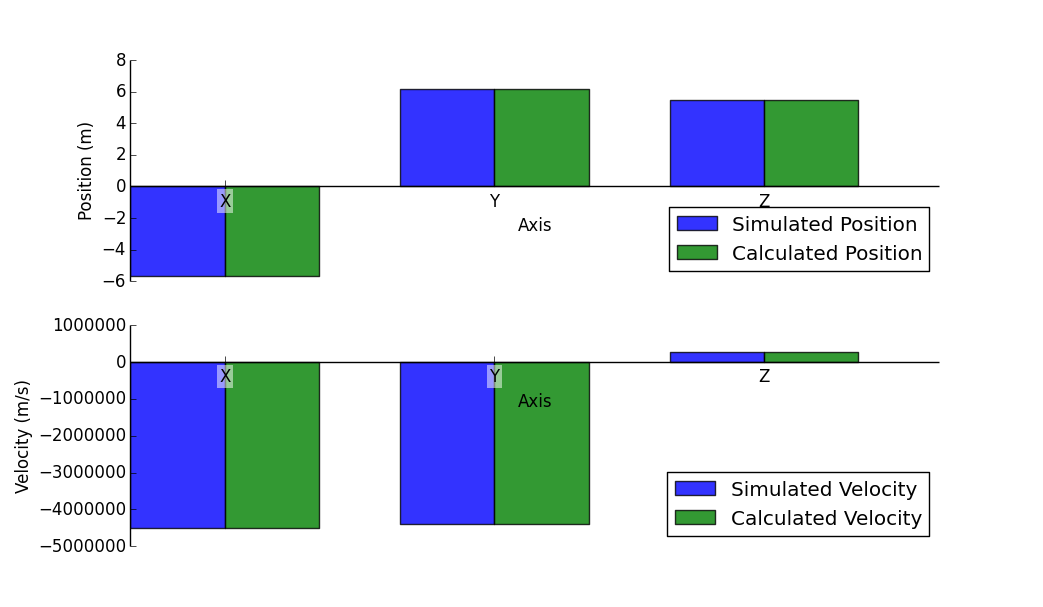
\includegraphics[width=0.5\textwidth]{Figures/IncCircCart_2.png}}
			\caption{Inclined Circular Orbit Varying $a$}
		\end{figure}
		\item \underline{Equatorial Circular Orbit ($e=0$,\quad $a>0$, \quad $\omega=0$, \quad $i=0$, \quad $\Omega=0$)}\\
		Like the inclined case, the only input varied for equatorial circular orbits is $a$. Also, all variations passed with no discrepancy, as shown in Fig. \ref{fig:7}.
		\begin{figure}[H]
			\centering
			\subfloat[$a=10^7$km]{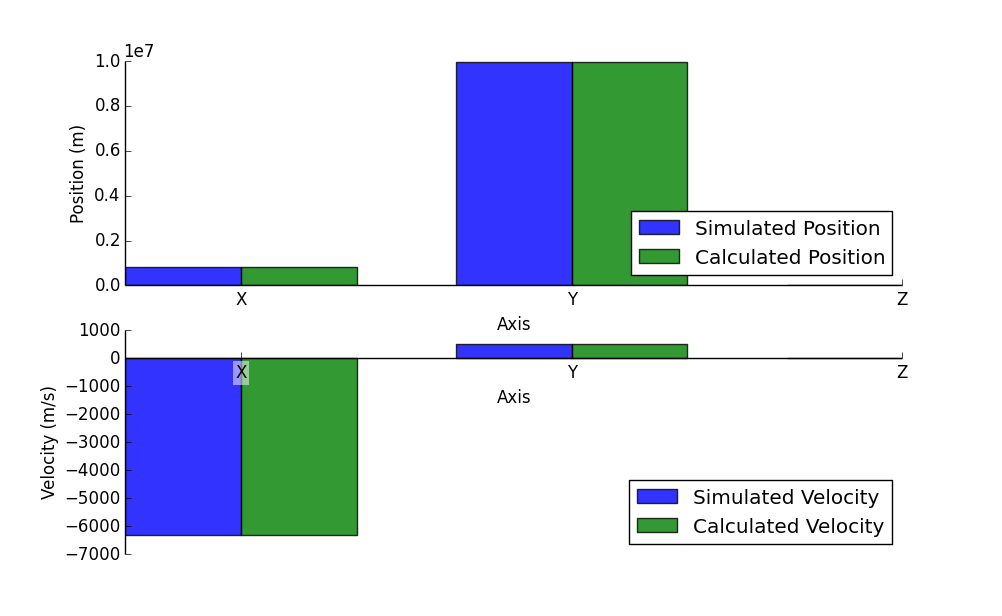
\includegraphics[width=0.5\textwidth]{Figures/EquCircCart_1.png}}
			\subfloat[$a=10$km]{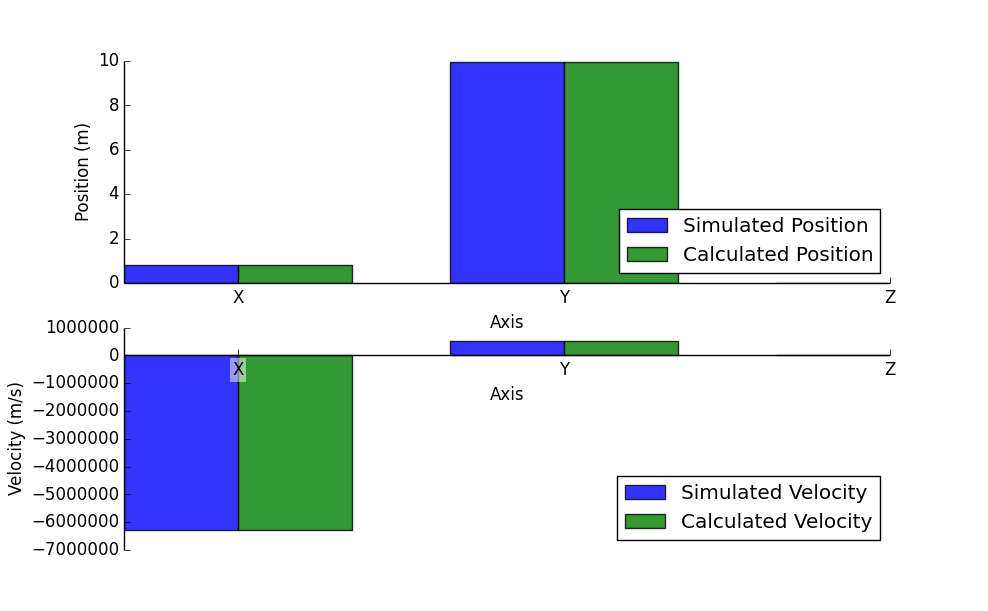
\includegraphics[width=0.5\textwidth]{Figures/EquCircCart_2.png}}
			\caption{Equatorial Circular Orbit Varying $a$}\label{fig:7}
		\end{figure}
		\pagebreak
		\item \underline{Inclined Parabolic Orbit ($e=1.0$, \quad $a=-r_p$)}\\
		For the parabolic orbit, the input is varied with $-10^5$km $<a < -10$km. As discussed in the model description, it is crucial that $a$ remains negative in the parabolic case. All variations passed for this case with discrepancies equal to zero displayed below.
		\begin{figure}[H] \label{fig:8}
			\centering
			\subfloat[$a=10^7$km]{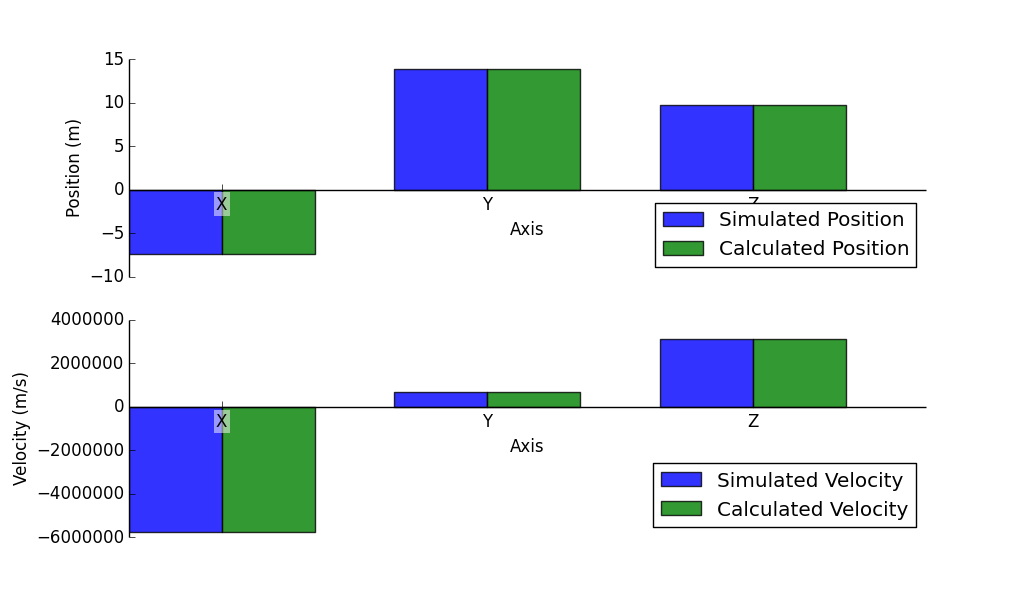
\includegraphics[width=0.5\textwidth]{Figures/IncParaCart_1.png}}
			\subfloat[$a=10$km]{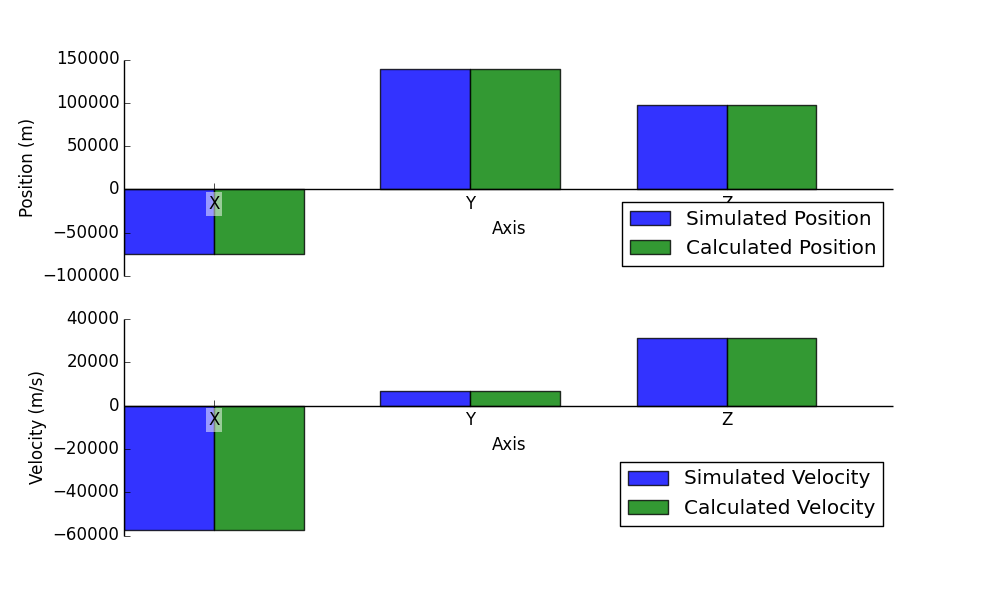
\includegraphics[width=0.5\textwidth]{Figures/IncParaCart_2.png}}
			\caption{Inclined Parabolic Orbit Varying $a$}
		\end{figure}
		\item \underline{Equatorial Parabolic Orbit ($e=1.0$, \quad $a=-r_p$, \quad $i=0$, \quad $\Omega=0$)}\\
		The equatorial parabolic orbit is tested with the same range of $a$ as the inclined case. This orbit also passed for all variations and the results are shown in Fig. \ref{fig:9}.
		\begin{figure}[H]
			\centering
			\subfloat[$a=10^7$km]{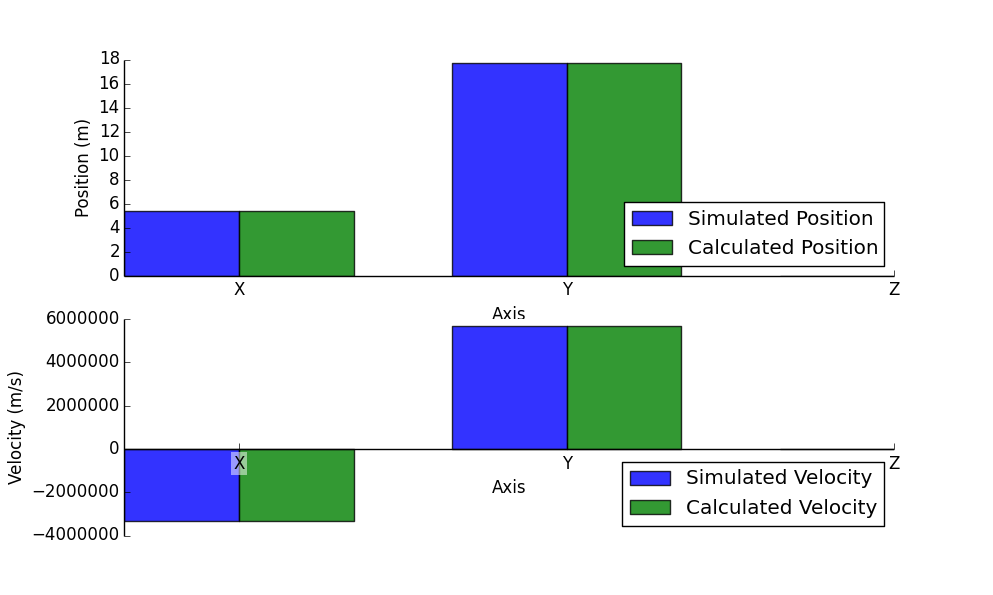
\includegraphics[width=0.5\textwidth]{Figures/EquParaCart_1.png}}
			\subfloat[$a=10$km]{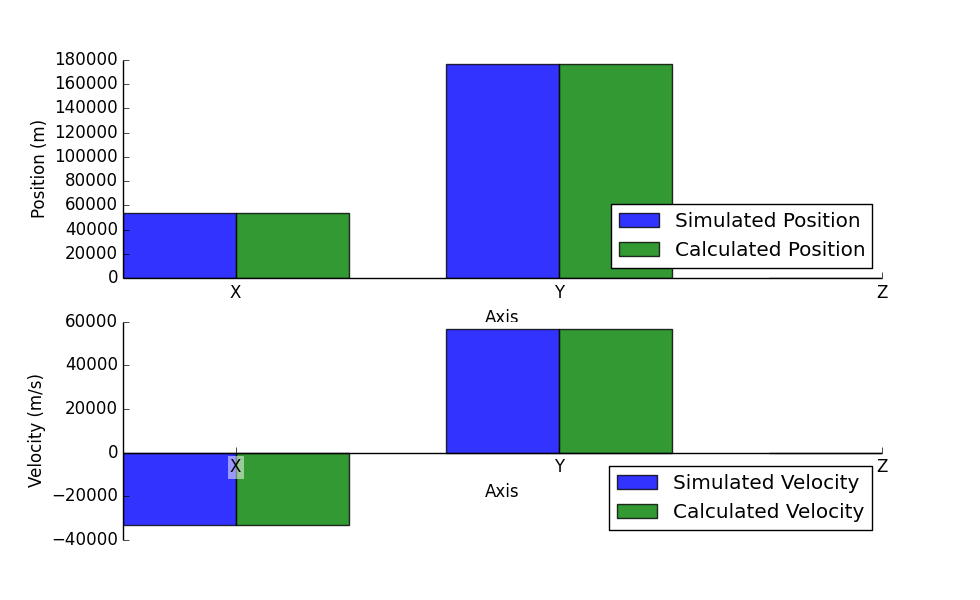
\includegraphics[width=0.5\textwidth]{Figures/EquParaCart_2.png}}
			\caption{Equatorial Parabolic Orbit Varying $a$}\label{fig:9}
		\end{figure}
		\pagebreak
		\item \underline{Inclined Hyperbolic Orbit ($e>1.0$, \quad $a<0$)}\\
		When testing hyperbolic orbits, $e$ and $a$ are both varied. While changing $e$ within the range $1.1<e<1.5$, $a=-10^4$km. While changing $a$ in the range $-10^5$km $<a < -10$km, $e=1.3$. All variations passed the tests, still with no discrepancies. The plots below compare the simulated and calculated results.
		\begin{figure}[H] \label{fig:10}
			\centering
			\subfloat[$e=1.1$, $a=-10^5$km]{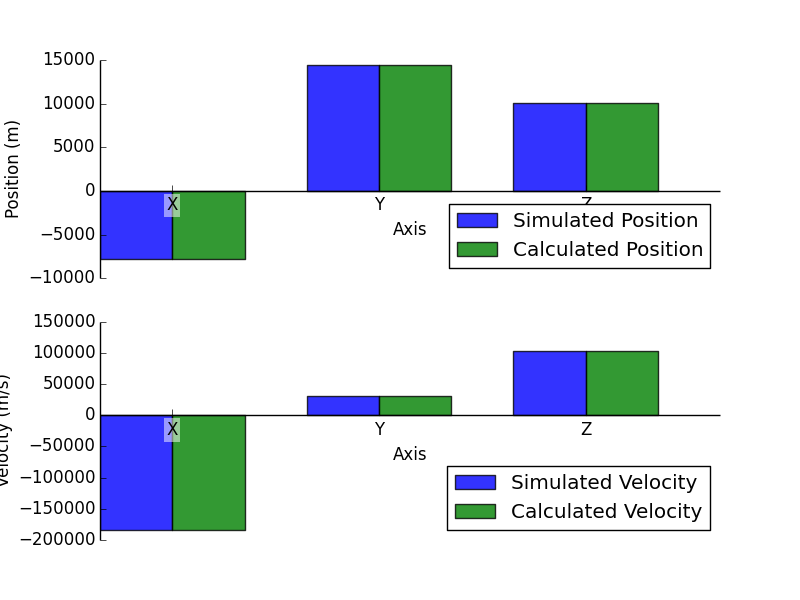
\includegraphics[width=0.5\textwidth]{Figures/IncHypCart_e_1.png}}
			\subfloat[$e=1.5$, $a=-10^5$km]{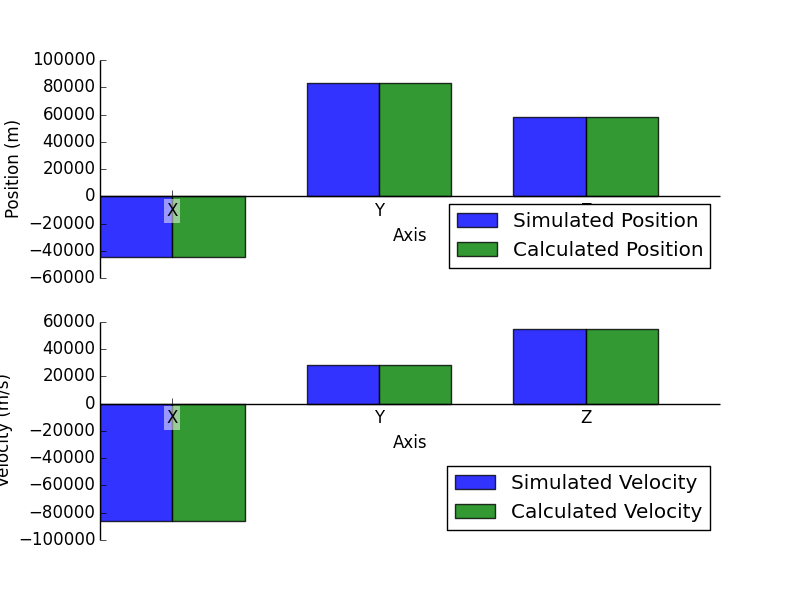
\includegraphics[width=0.5\textwidth]{Figures/IncHypCart_e_2.png}}
			\caption{Inclined Hyperbolic Orbit Varying $e$}
		\end{figure}
		\begin{figure}[H] \label{fig:11}
			\centering
			\subfloat[$e=1.3$, $a=-10$km]{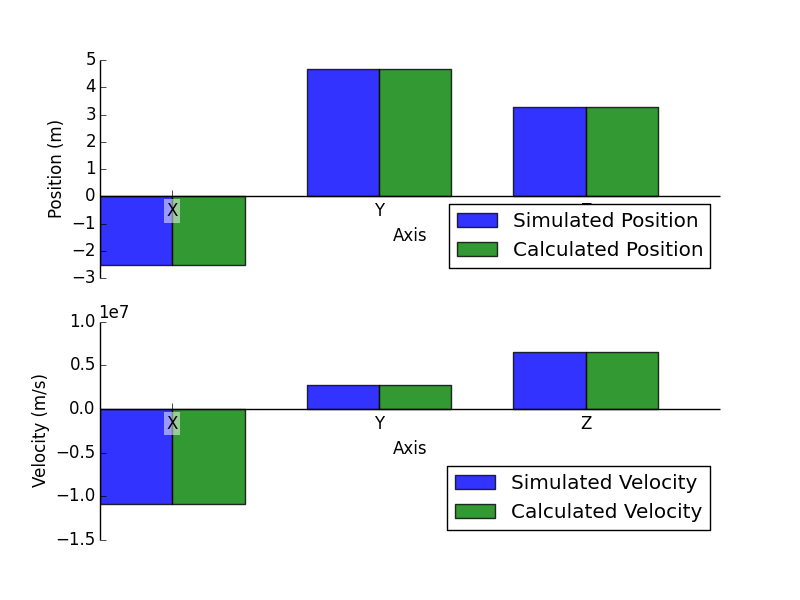
\includegraphics[width=0.5\textwidth]{Figures/IncHypCart_a_1.png}}
			\subfloat[$e=1.3$, $a=-10^5$km]{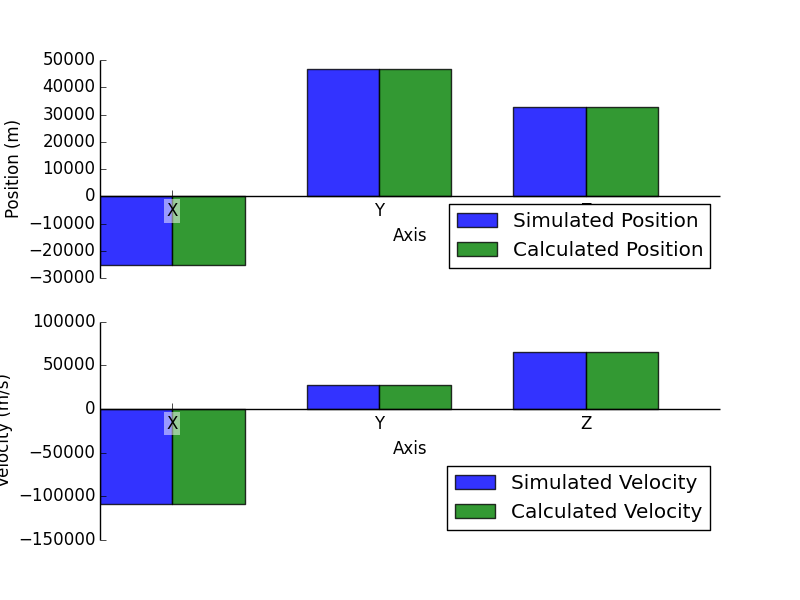
\includegraphics[width=0.5\textwidth]{Figures/IncHypCart_a_2.png}}
			\caption{Inclined Hyperbolic Orbit Varying $a$}
		\end{figure}
		\pagebreak
		\item \underline{Equatoral Hyperbolic Orbit ($e>1.0$, \quad $a<0$, \quad $i=0$, \quad $\Omega = 0$)}\\
		Equatorial hyperbolic orbits are tested with the same range of $e$ and $a$ inputs as the inclined case. Also, all variations passed without discrepancy, as shown in the following Fig. \ref{fig:12} and \ref{fig:13}:
		\begin{figure}[H]
			\centering
			\subfloat[$e=1.1$,$a=-10^5$km]{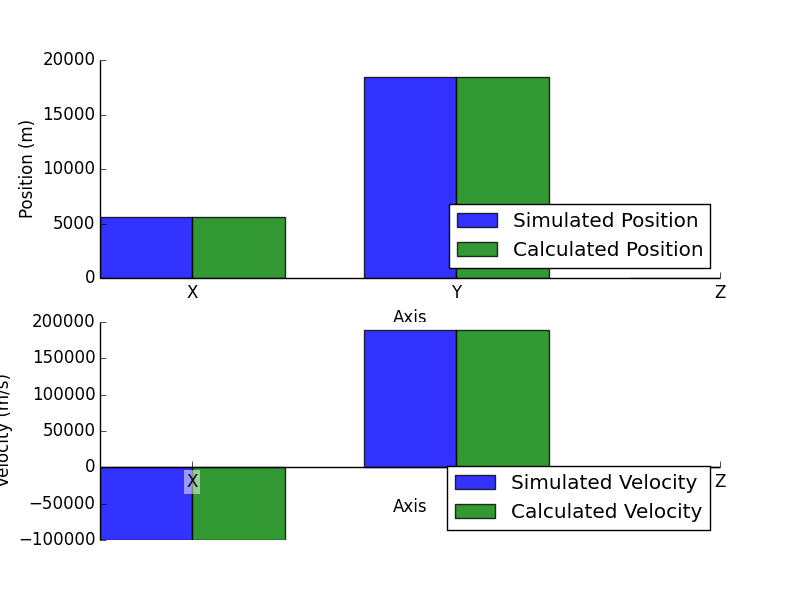
\includegraphics[width=0.5\textwidth]{Figures/EquHypCart_e_1.png}}
			\subfloat[$e=1.5$, $a=-10^5$km]{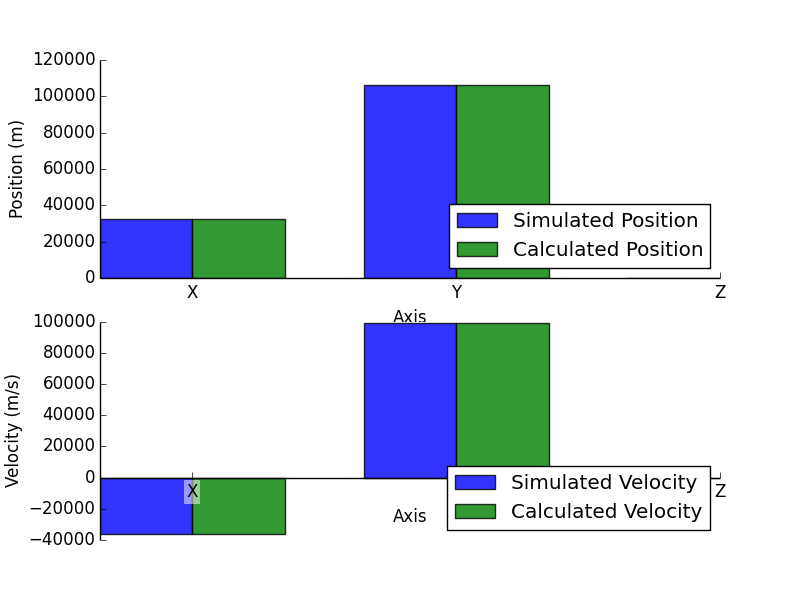
\includegraphics[width=0.5\textwidth]{Figures/EquHypCart_e_2.png}}
			\caption{Equatorial Hyperbolic Orbit Varying $e$}\label{fig:12}
		\end{figure}
		\begin{figure}[H]
			\centering
			\subfloat[$e=1.3$, $a=-10$km]{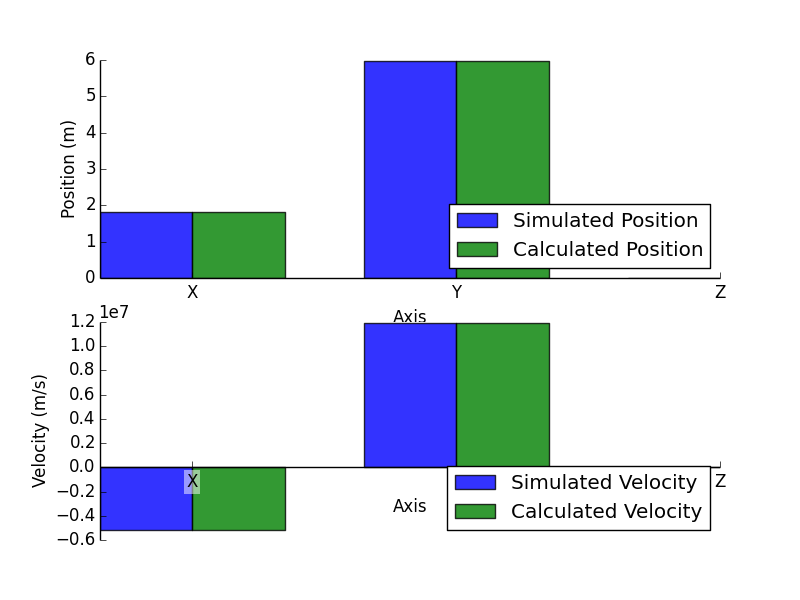
\includegraphics[width=0.5\textwidth]{Figures/EquHypCart_a_1.png}}
			\subfloat[$e=1.3$, $a=-10^5$km]{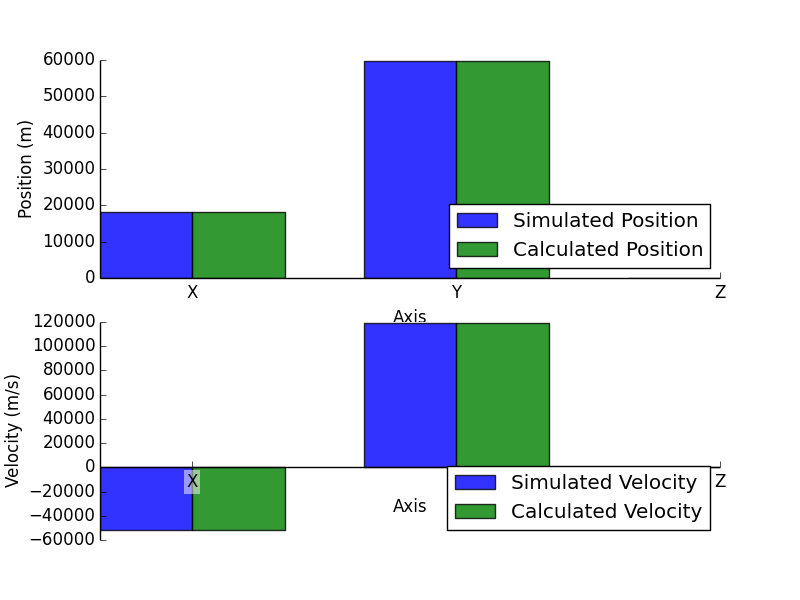
\includegraphics[width=0.5\textwidth]{Figures/EquHypCart_a_2.png}}
			\caption{Equatorial Hyperbolic Orbit Varying $a$}\label{fig:13}
		\end{figure}
	\end{enumerate}
	\pagebreak
	\item \textbf{Cartesian to Element}\\
	\begin{table}[H]
		\caption{Cartesian to Element Test Results}
		\label{tab:Elem to Cart results}
		\centering \fontsize{10}{10}\selectfont
		\begin{tabular}{c|c|c} % Column formatting, 
			\hline
			\textbf{Parameter Sets} & \textbf{Results} & \textbf{Notes} 									\\ \hline
			1 & \color{Green}{PASSED} & NA\\
			2 & \color{Green}{PASSED} & NA\\
			3 & \color{Green}{PASSED} & NA\\
			4 & \color{Green}{PASSED} & NA\\
			5 & \color{Green}{PASSED} & NA\\
			6 & \color{Green}{PASSED} & NA\\
			7 & \color{Green}{PASSED} & NA\\
			8 & \color{Green}{PASSED} & NA\\
			\hline
		\end{tabular}
		%		Setup Test 		   			  	& \input{AutoTex/sphericalHarmonicsPassFail}     & \input{AutoTex/sphericalHarmonicsFailMsg}			 \\ \hline
		%		Single-Body Gravity		   	& \input{AutoTex/singleBodyPassFail}                 & \input{AutoTex/singleBodyFailMsg} \\ \hline
		%		Multi-Body Gravity			 &\input{AutoTex/multiBodyPassFail}  			 	 &  \input{AutoTex/multiBodyFailMsg} 			   \\ \hline
	\end{table}
	Orbital elements are tested by making two comparisons. The first compares the simulated output with the calculated output, like in the previous conversion. The second compares elements initially used as inputs for the first conversion with those produced as the output of the second. As observed when testing the previous conversion, the comparison between calculated and simulated elements results in complete agreement. Also, the two cases presented by the astronomical body identifier, once again, produce identical results. Thus, the main focus of the Cartesian to element test results is the input/output comparison.
	
	Displayed below are explanations of the results after converting Cartesian to elements. Graphical representations of the parameter comparisons for each orbit type are not provided for this test, since the output is already specified above as the input when converting from elements to Cartesian. Figures from above can also be referenced for the Cartesian inputs. 
	
	\begin{enumerate}
		\item \underline{Inclined Elliptic Orbit ($0<e<1.0$,\quad $a>0$)}\\
		All variations passed the tests performed, however, the discrepancy between semimajor axis initial input and simulated result increases as eccentricity approaches 1.0. This is because it approaches the parabolic case, which requires a different conversion method and makes the elliptic calculations less accurate. The discrepancy with the tested parameters never increases past $10^{-7}$km, though, and since the semimajor axis is typically on the scale of at least $10^7$km, this is acceptable. Fig. \ref{fig:aDiff} shows the change in semimajor axis discrepancy as eccentricity reaches 0.999. %and Figures \ref{fig:14} and \ref{fig:15} illustrate the test results.
		\begin{figure} [H]
			\centering
			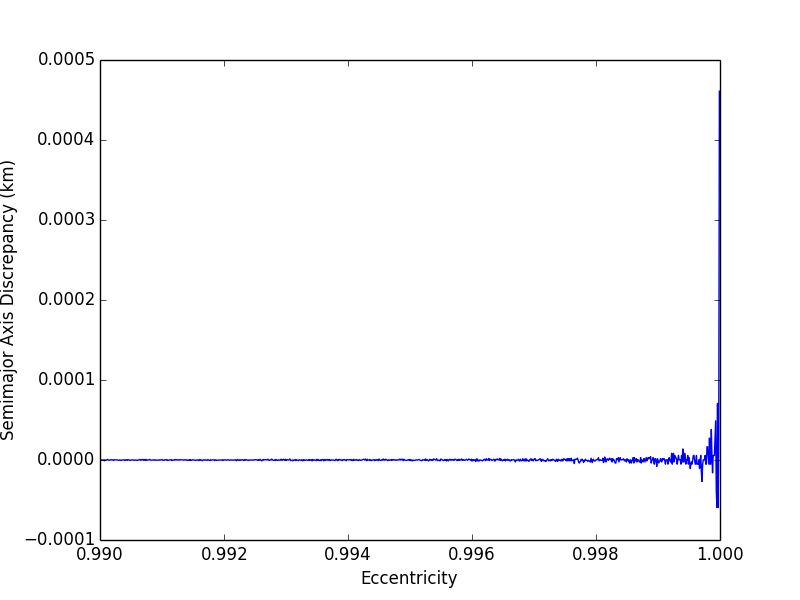
\includegraphics[width=0.5\textwidth]{Figures/aDiff.png}
			\caption{Input/Output Discrepancy for Semimajor Axis as Eccentricity Approaches 1.0}\label{fig:aDiff}
		\end{figure}
		%		\begin{figure}[H]
		%			\centering
		%			\subfloat[$e=0.01$ and $a=10^7$km]{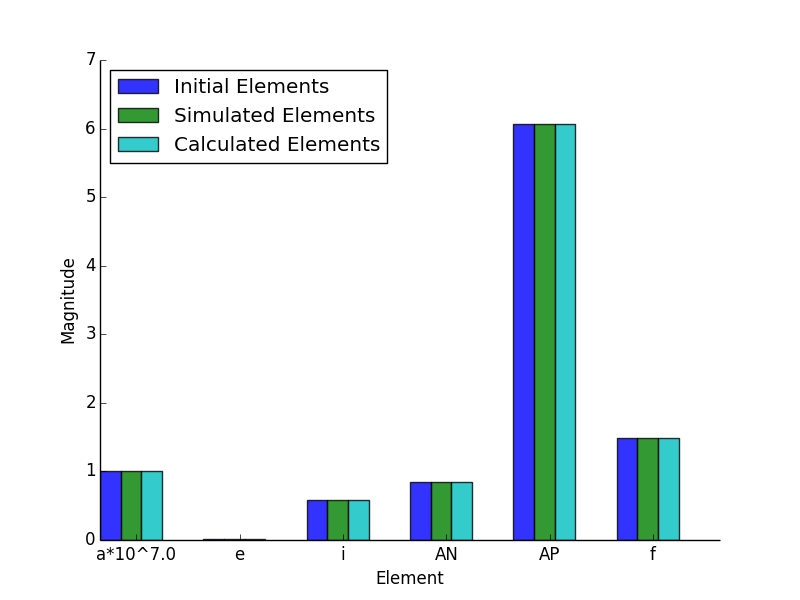
\includegraphics[width=0.5\textwidth]{Figures/IncEllipElem_e_1.png}}
		%			\subfloat[$e=0.75$ and $a=10^7$km]{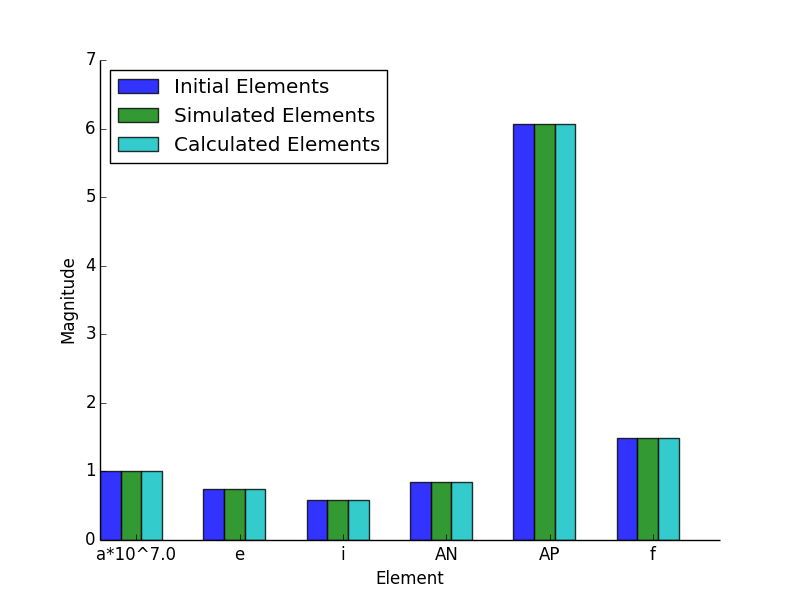
\includegraphics[width=0.5\textwidth]{Figures/IncEllipElem_e_2.png}}
		%			\caption{Inclined Elliptical Orbit Varying $e$}\label{fig:14}
		%		\end{figure}
		%		\begin{figure}[H]
		%			\centering
		%			\subfloat[$e=0.5$ and $a=10^7$km]{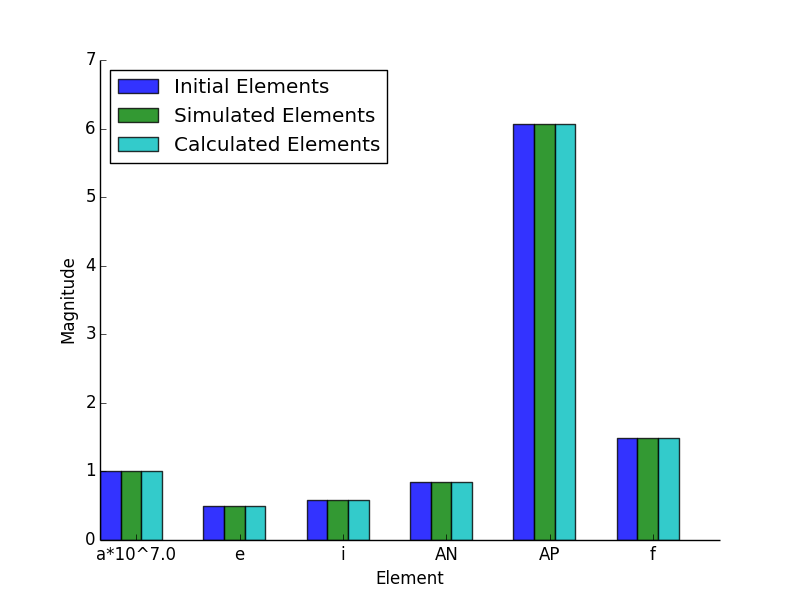
\includegraphics[width=0.5\textwidth]{Figures/IncEllipElem_a_1.png}}
		%			\subfloat[$e=0.5$ and $a=10$km]{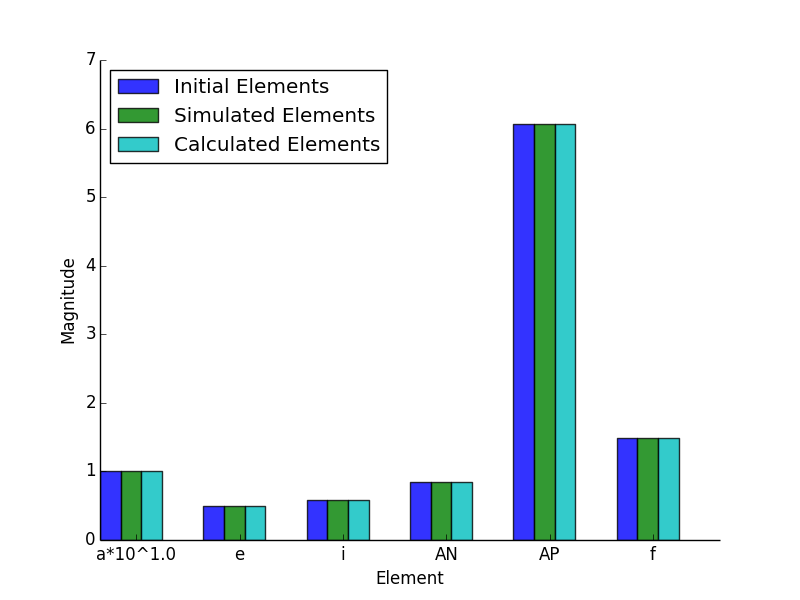
\includegraphics[width=0.5\textwidth]{Figures/IncEllipElem_a_2.png}}
		%			\caption{Inclined Elliptical Orbit Varying $a$}\label{fig:15}
		%		\end{figure}
		%\pagebreak
		\item \underline{Equatorial Elliptic Orbit ($0<e<1.0$,\quad $a>0$,\quad $i=0$,\quad $\Omega=0$)}\\
		All variations also passed for this case with much lower discrepancies than the previous one, due to the initial input $e=0.5$. The largest difference still occurs when comparing the semimajor axis, but this time it only reaches $10^{-15}$km. %The figures below display the output parameters.
		%		\begin{figure}[H] \label{fig:16}
		%			\centering
		%			\subfloat[$e=0.01$ and $a=10^7$km]{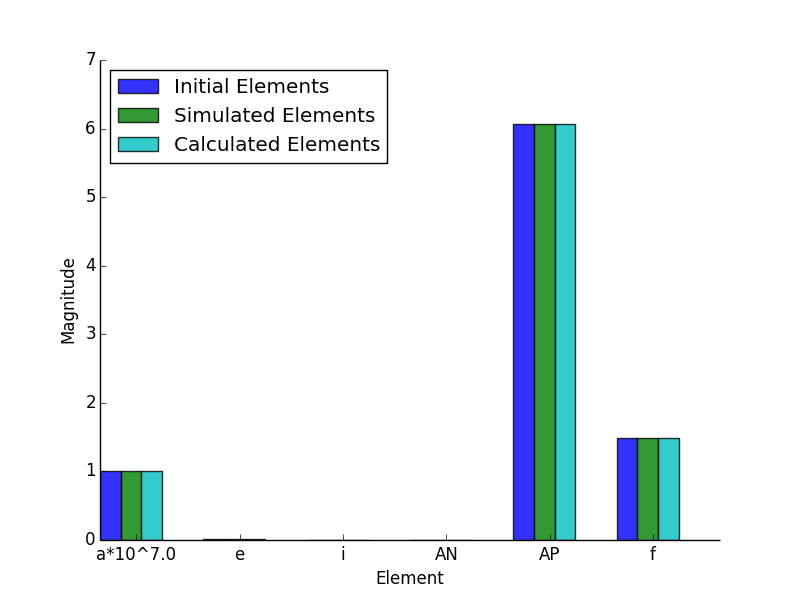
\includegraphics[width=0.5\textwidth]{Figures/EquEllipElem_e_1.png}}
		%			\subfloat[$e=0.75$ and $a=10^7$km]{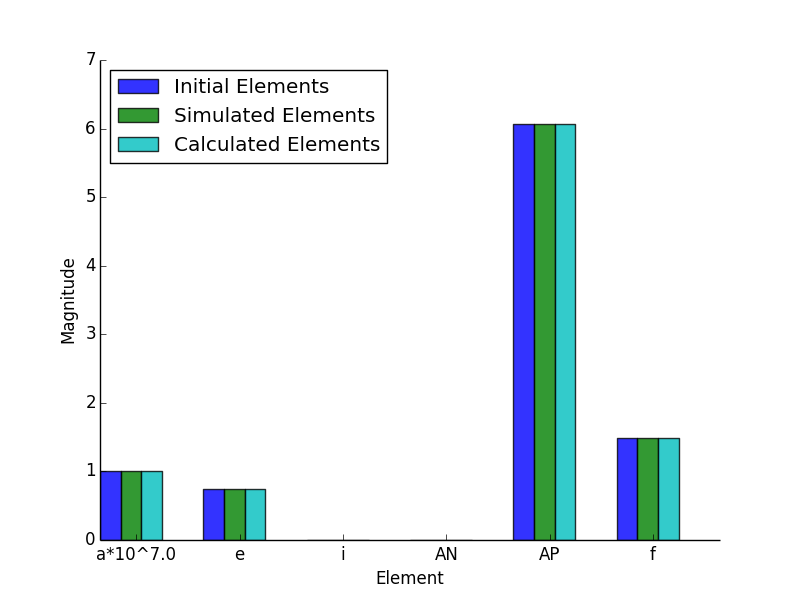
\includegraphics[width=0.5\textwidth]{Figures/EquEllipElem_e_2.png}}
		%			\caption{Equatorial Elliptical Orbit Varying $e$}
		%		\end{figure}
		%		\begin{figure}[H] \label{fig:17}
		%			\centering
		%			\subfloat[$e=0.5$ and $a=10^7$km]{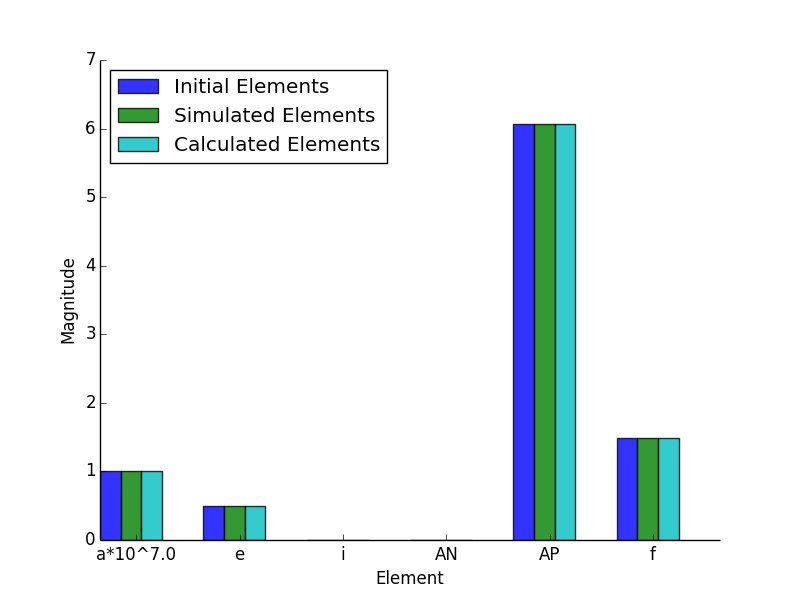
\includegraphics[width=0.5\textwidth]{Figures/EquEllipElem_a_1.png}}
		%			\subfloat[$e=0.5$ and $a=10$km]{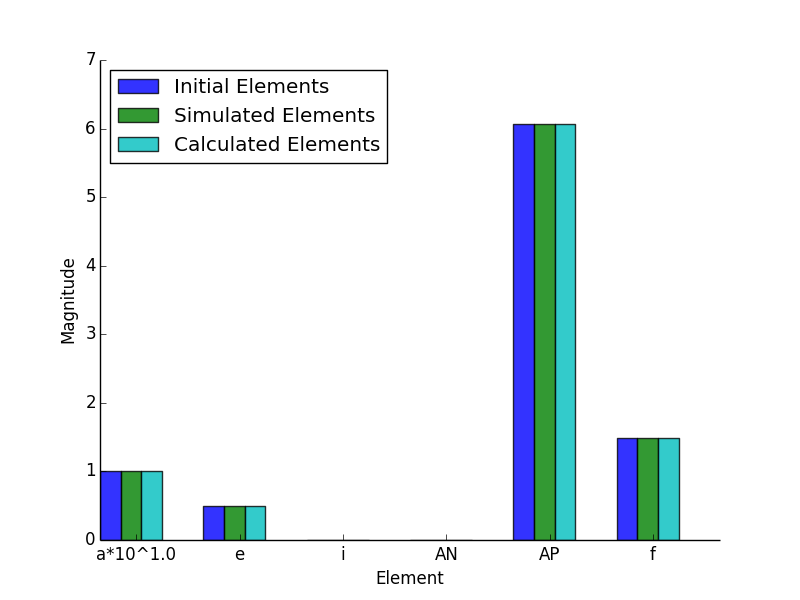
\includegraphics[width=0.5\textwidth]{Figures/EquEllipElem_a_2.png}}
		%			\caption{Equatorial Elliptical Orbit Varying $a$}
		%		\end{figure}
		%		\pagebreak
		\item \underline{Inclined Circular Orbit ($e=0$, \quad $a>0$,\quad $\omega=0$)}\\
		All variations passed in the inclined circular orbit tests with the maximum tolerance at about $10^{-9}$. As initial input $a$ decreases, so does the tolerance, resulting in no discrepancy when $a=10$km. %The comparisons are shown below.
		%		\begin{figure}[H]
		%			\centering
		%			\subfloat[$a=10^7$km]{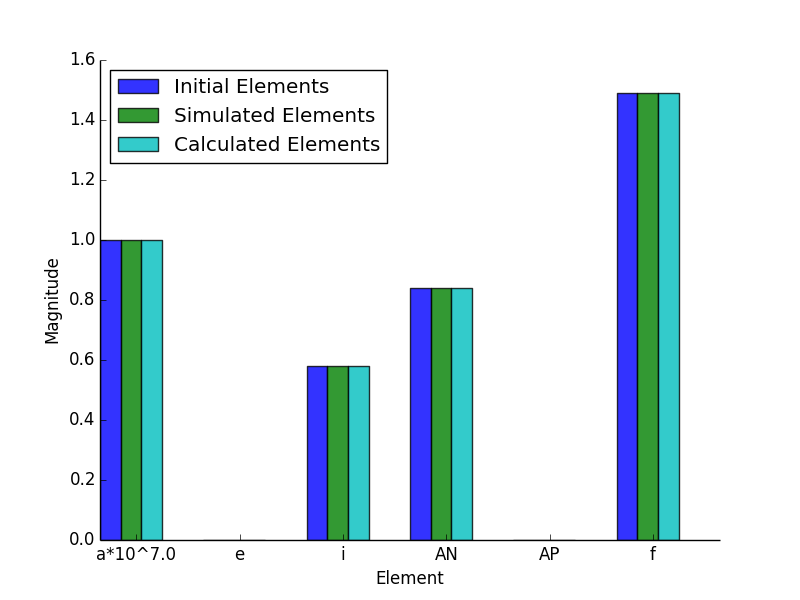
\includegraphics[width=0.5\textwidth]{Figures/IncCircElem_1.png}}
		%			\subfloat[$a=10$km]{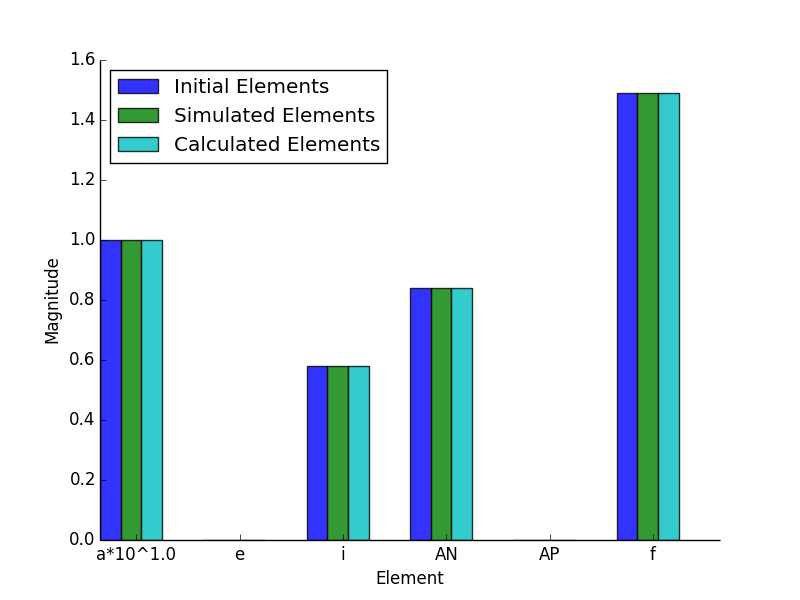
\includegraphics[width=0.5\textwidth]{Figures/IncCircElem_2.png}}
		%			\caption{Inclined Circular Orbit Varying $a$}
		%		\end{figure}
		\item \underline{Equatorial Circular Orbit ($e=0$,\quad $a>0$, \quad $\omega=0$, \quad $i=0$, \quad $\Omega=0$)}\\
		All variations passed as well, this time resulting in a tolerance of zero for almost all parameters. The only non-zero discrepancy is eccentricity with a difference of $10^{-17}$ between input and output. %Figure \ref{fig:19}  compares the orbital elements for the equatorial circular orbit.
		%		\begin{figure}[H]
		%			\centering
		%			\subfloat[$a=10^7$km]{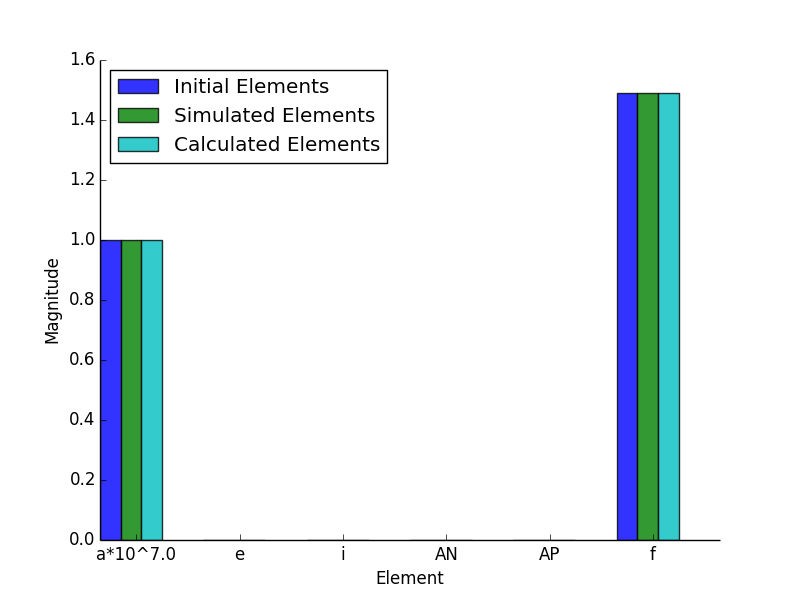
\includegraphics[width=0.5\textwidth]{Figures/EquCircElem_1.png}}
		%			\subfloat[$a=10$km]{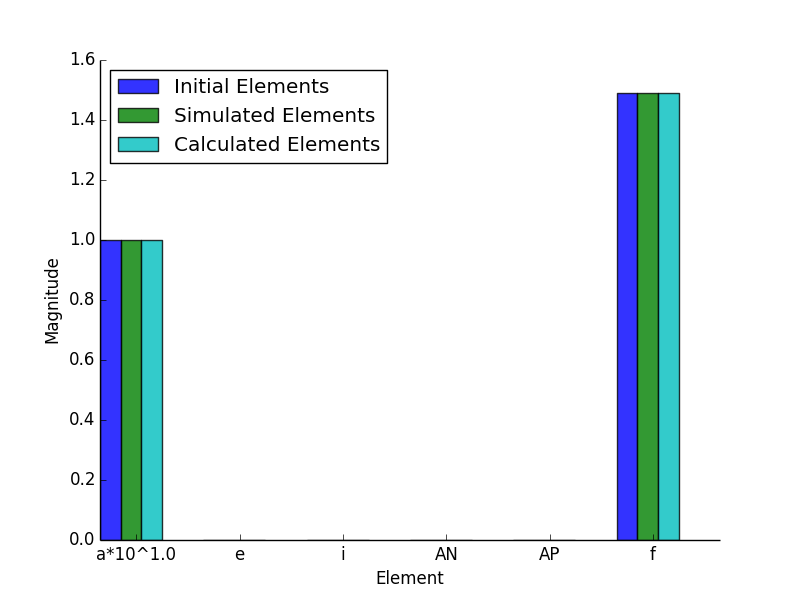
\includegraphics[width=0.5\textwidth]{Figures/EquCircElem_2.png}}
		%			\caption{Equatorial Circular Orbit Varying $a$}\label{fig:19}
		%		\end{figure}
		%		\pagebreak
		\item \underline{Inclined Parabolic Orbit ($e=1.0$, \quad $a=-r_p$)}\\
		All variations passed for this orbit with tolerances well below the maximum allowed and decreasing as initial input $a$ becomes more negative. %The following figure shows the parameter comparisons.
		%		\begin{figure}[H]
		%			\centering
		%			\subfloat[$a=-10$km]{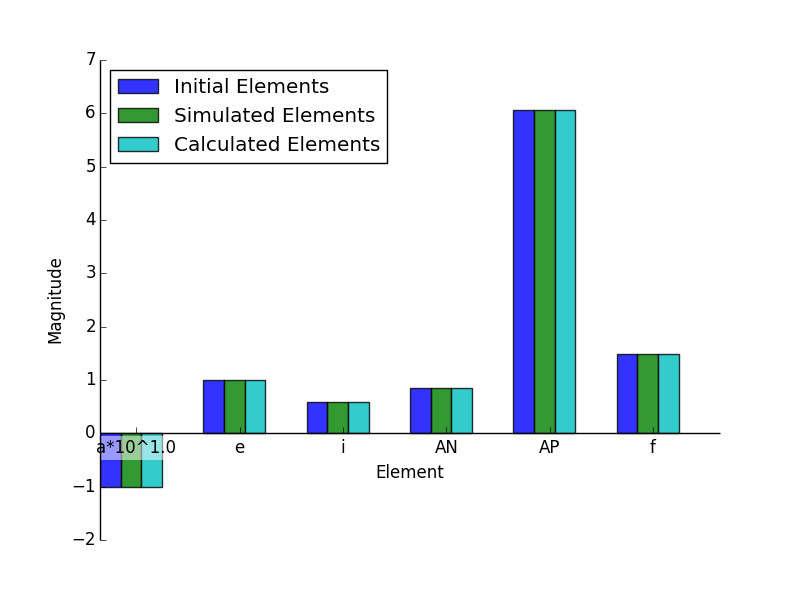
\includegraphics[width=0.5\textwidth]{Figures/IncParaElem_1.png}}
		%			\subfloat[$a=-10^5$km]{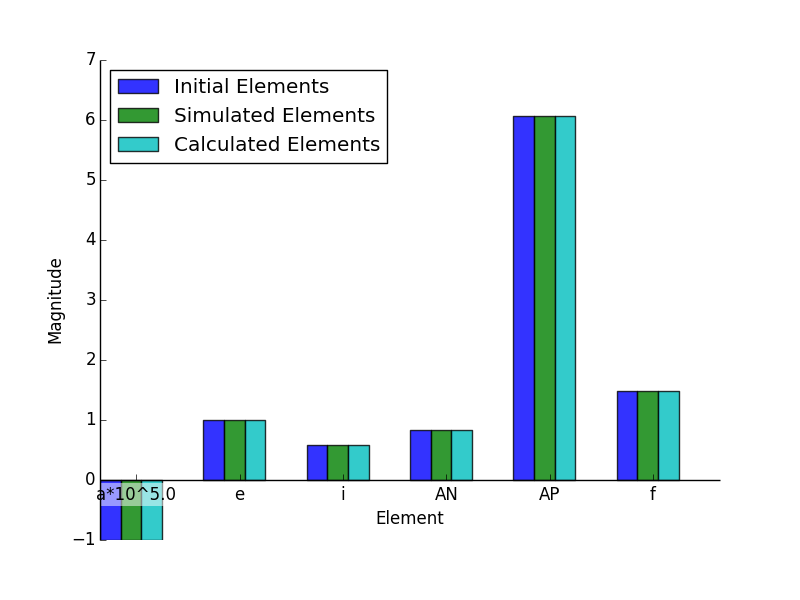
\includegraphics[width=0.5\textwidth]{Figures/IncParaElem_2.png}}
		%			\caption{Inclined Parabolic Orbit Varying $a$}
		%		\end{figure}
		\item \underline{Equatorial Parabolic Orbit ($e=1.0$, \quad $a=-r_p$, \quad $i=0$, \quad $\Omega=0$)}\\
		This orbit also passed for all variations with discrepancies similar to those seen in the inclined case. %Figure \ref{fig:21} illustrates these results:
		%		\begin{figure}[H]
		%			\centering
		%			\subfloat[$a=-10$km]{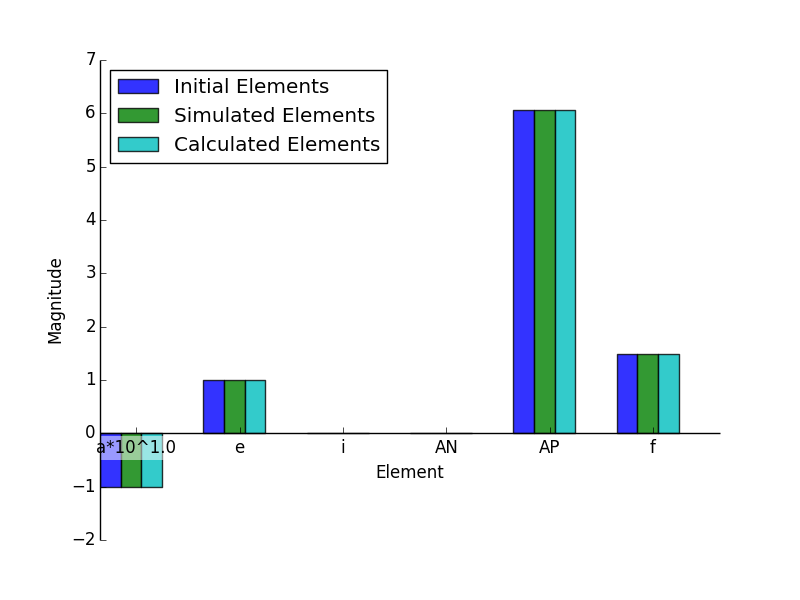
\includegraphics[width=0.5\textwidth]{Figures/EquParaElem_1.png}}
		%			\subfloat[$a=-10^5$km]{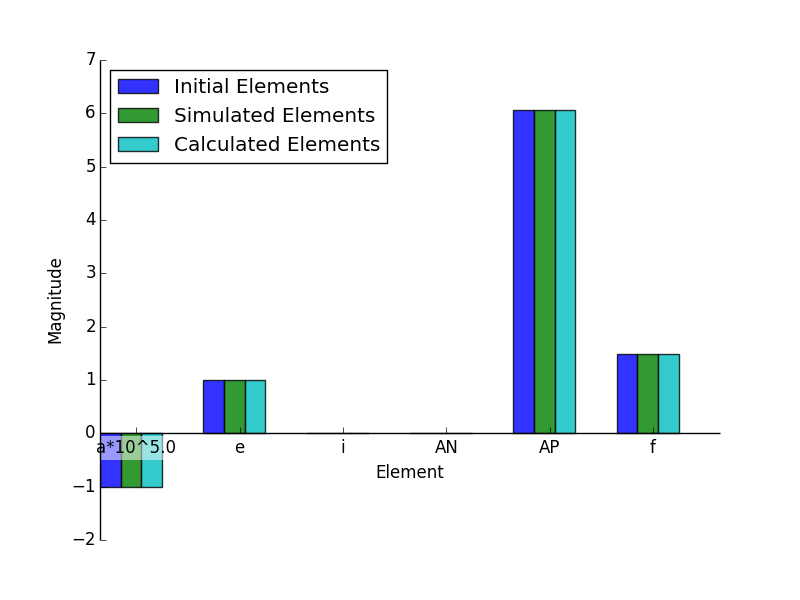
\includegraphics[width=0.5\textwidth]{Figures/EquParaElem_2.png}}
		%			\caption{Equatorial Parabolic Orbit Varying $a$}\label{fig:21}
		%		\end{figure}
		%		\pagebreak
		\item \underline{Inclined Hyperbolic Orbit ($e>1.0$, \quad $a<0$)}\\
		All tests passed with discrepancies well below the maximum limit. %as shown in the figures below.
		%		\begin{figure}[H]
		%			\centering
		%			\subfloat[$e=1.1$, $a=-10^5$km]{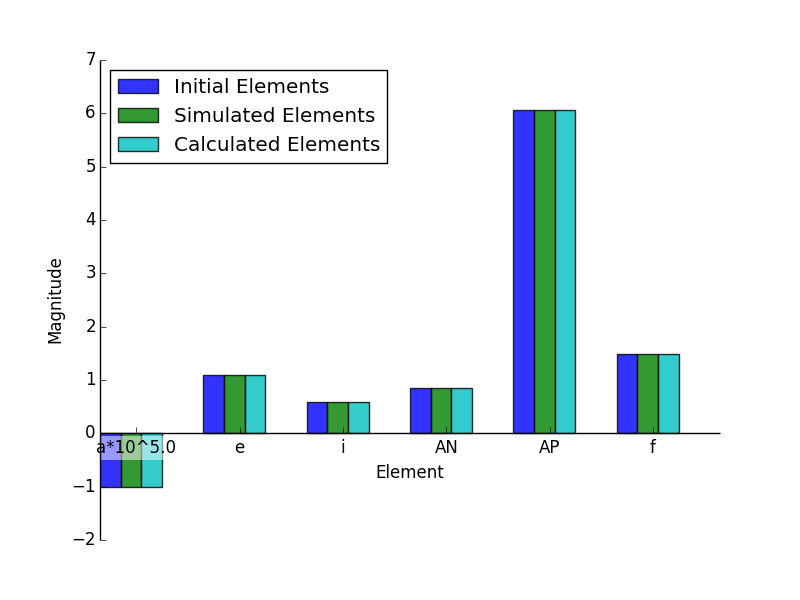
\includegraphics[width=0.5\textwidth]{Figures/IncHypElem_e_1.png}}
		%			\subfloat[$e=1.5$, $a=-10^5$km]{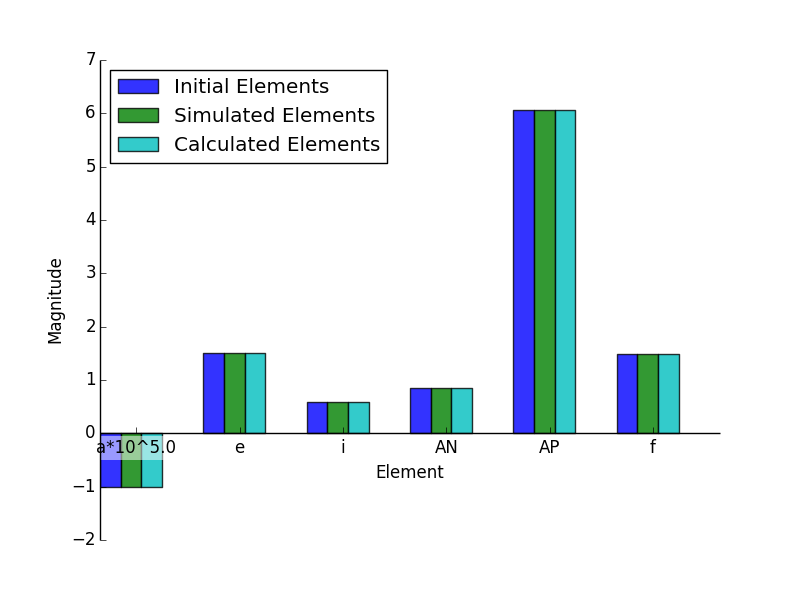
\includegraphics[width=0.5\textwidth]{Figures/IncHypElem_e_2.png}}
		%			\caption{Inclined Hyperbolic Orbit Varying $e$}
		%		\end{figure}
		%		\begin{figure}[H]
		%			\centering
		%			\subfloat[$e=1.3$, $a=-10$km]{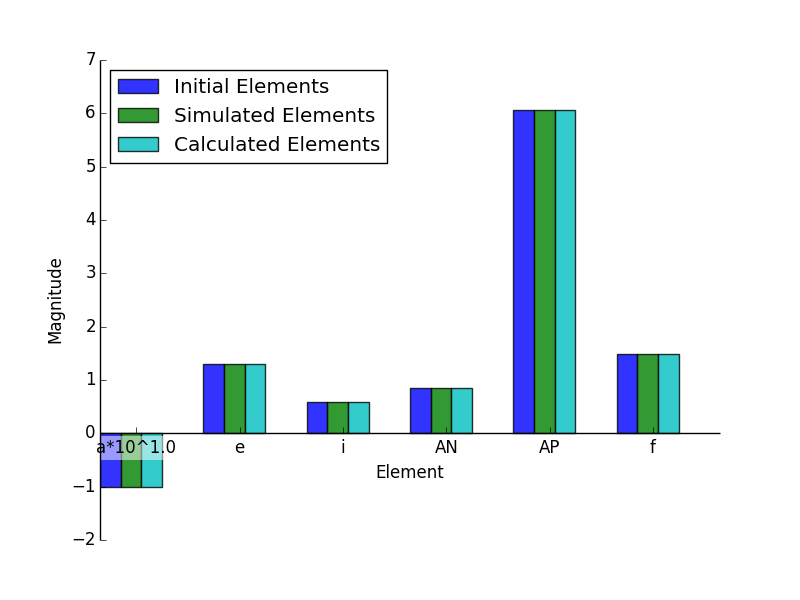
\includegraphics[width=0.5\textwidth]{Figures/IncHypElem_a_1.png}}
		%			\subfloat[$e=1.3$, $a=-10^5$km]{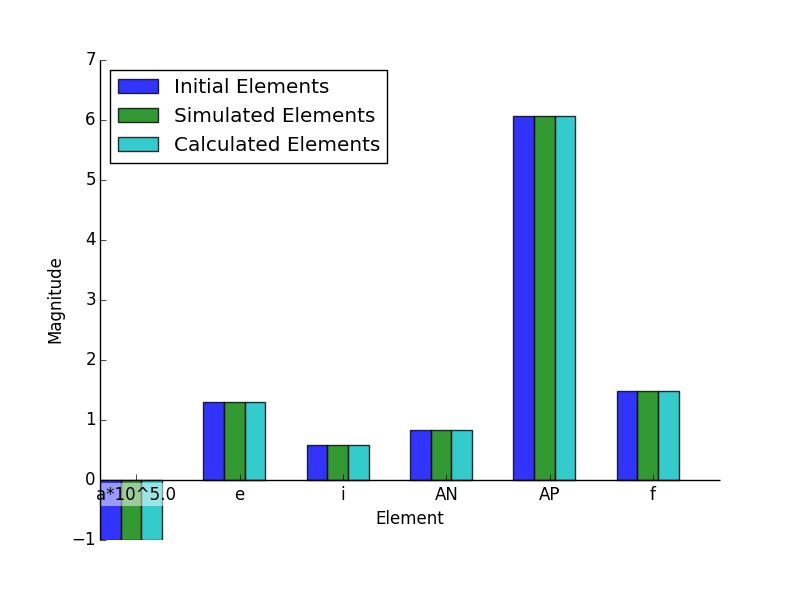
\includegraphics[width=0.5\textwidth]{Figures/IncHypElem_a_2.png}}
		%			\caption{Inclined Hyperbolic Orbit Varying $a$}
		%		\end{figure}
		%		\pagebreak
		\item \underline{Equatorial Hyperbolic Orbit ($e>1.0$, \quad $a<0$, \quad $i=0$, \quad $\Omega = 0$)}\\
		Each variation passed when tested, satisfying the tolerance limitation. The equatorial case exhibits lesser discrepancies than the inclined. %and the results are shown in figures \ref{fig:24} and \ref{fig:25}.
		%		\begin{figure}[H]
		%			\centering
		%			\subfloat[$a=-10$km]{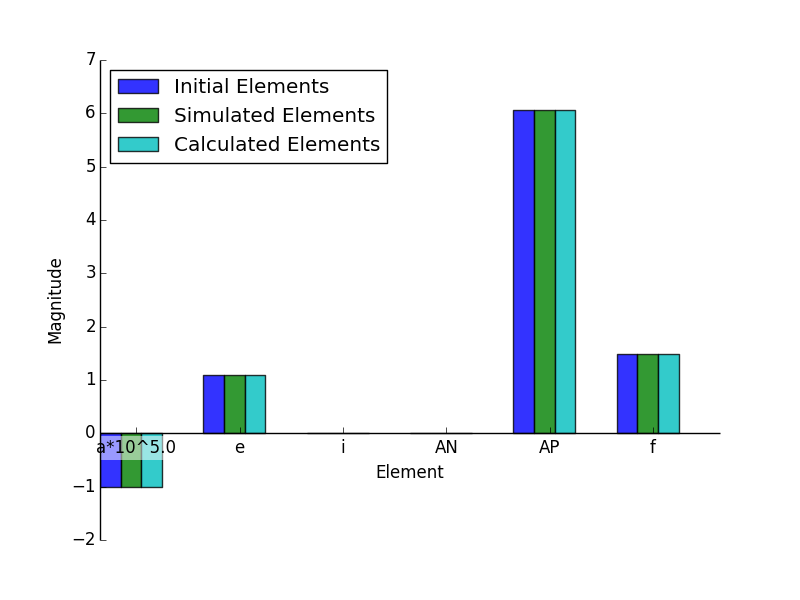
\includegraphics[width=0.5\textwidth]{Figures/EquHypElem_e_1.png}}
		%			\subfloat[$a=-10^5$km]{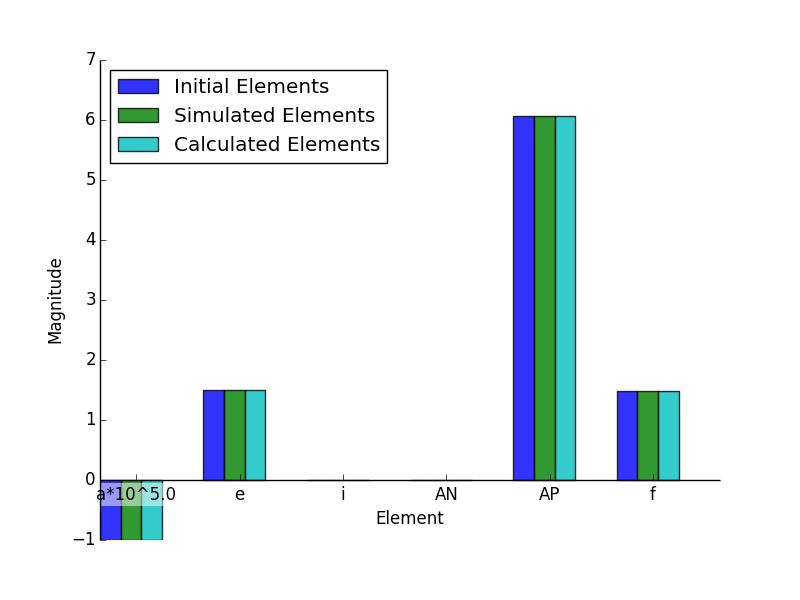
\includegraphics[width=0.5\textwidth]{Figures/EquHypElem_e_2.png}}
		%			\caption{Equatorial Hyperbolic Orbit Varying $a$}\label{fig:24}
		%		\end{figure}
		%		\begin{figure}[H]
		%			\centering
		%			\subfloat[$e=1.3$, $a=-10$km]{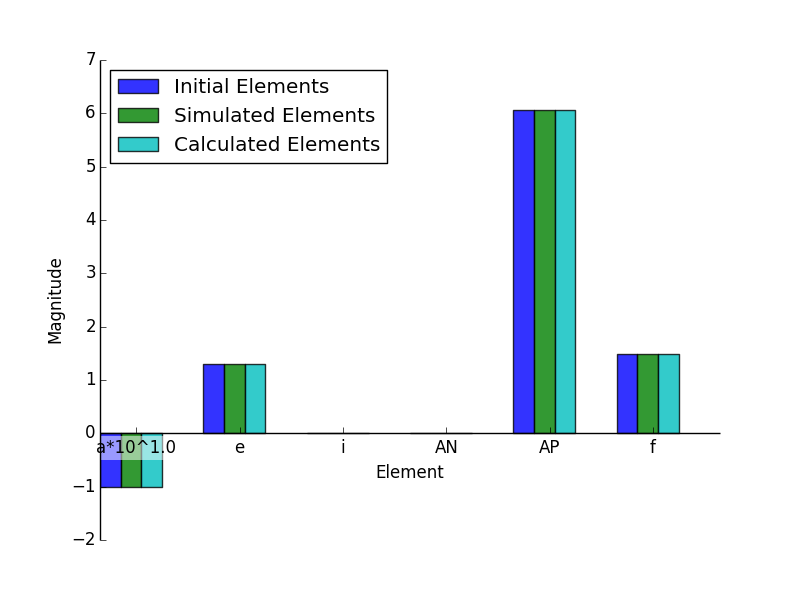
\includegraphics[width=0.5\textwidth]{Figures/EquHypElem_a_1.png}}
		%			\subfloat[$e=1.3$, $a=-10^5$km]{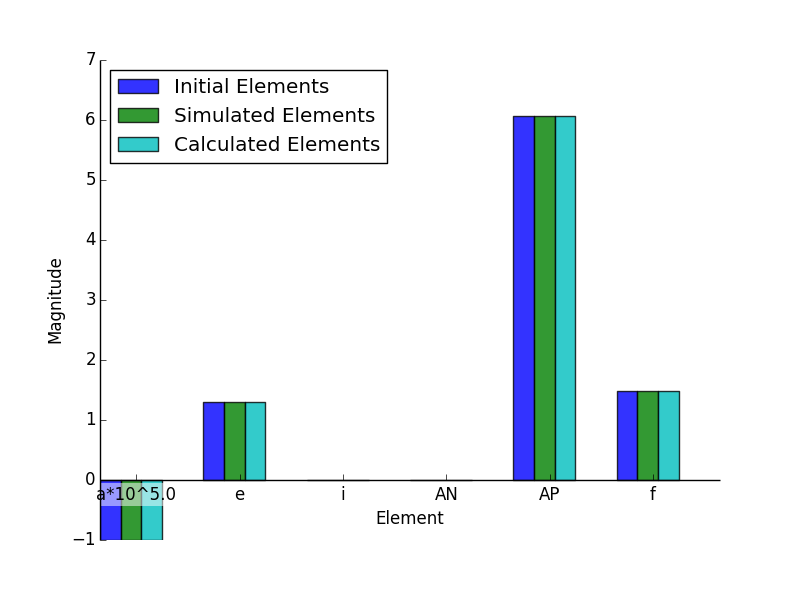
\includegraphics[width=0.5\textwidth]{Figures/EquHypElem_a_2.png}}
		%			\caption{Equatorial Hyperbolic Orbit Varying $e$}\label{fig:25}
		%		\end{figure}
	\end{enumerate}
\end{itemize}
\pagebreak